% !TEX root = main.tex

\subsection{Comparison to the Electricity Mix}
\label{ch:elecMix}

Comparing the emission factor with the emission factors of the electricity mix of other countries enables us to identify where technologies like the ASF would be best suited. In Switzerland where the simulation was run, we see a 6\% reduction compared to the average electricity mix. This is because the Swiss electricity mix is dominated by Hydro and Nuclear which has a very low GWP potential. Germany on the otherhand, the ASF has a 81\% reduction in carbon emissions. \\

[Graph of Switzerland, Germany, France, China and the USA]


\subsection{Comparison to other technologies}

Comparison of the ASF to other PV technologies and the UCTE electricity mix is highlighted in Figure \ref{fig:compPV}. The ASF outperforms the silicon technologies, however is still inferior to simply mounted static CIGS panels. 


\begin{figure}[H]
\begin{center}
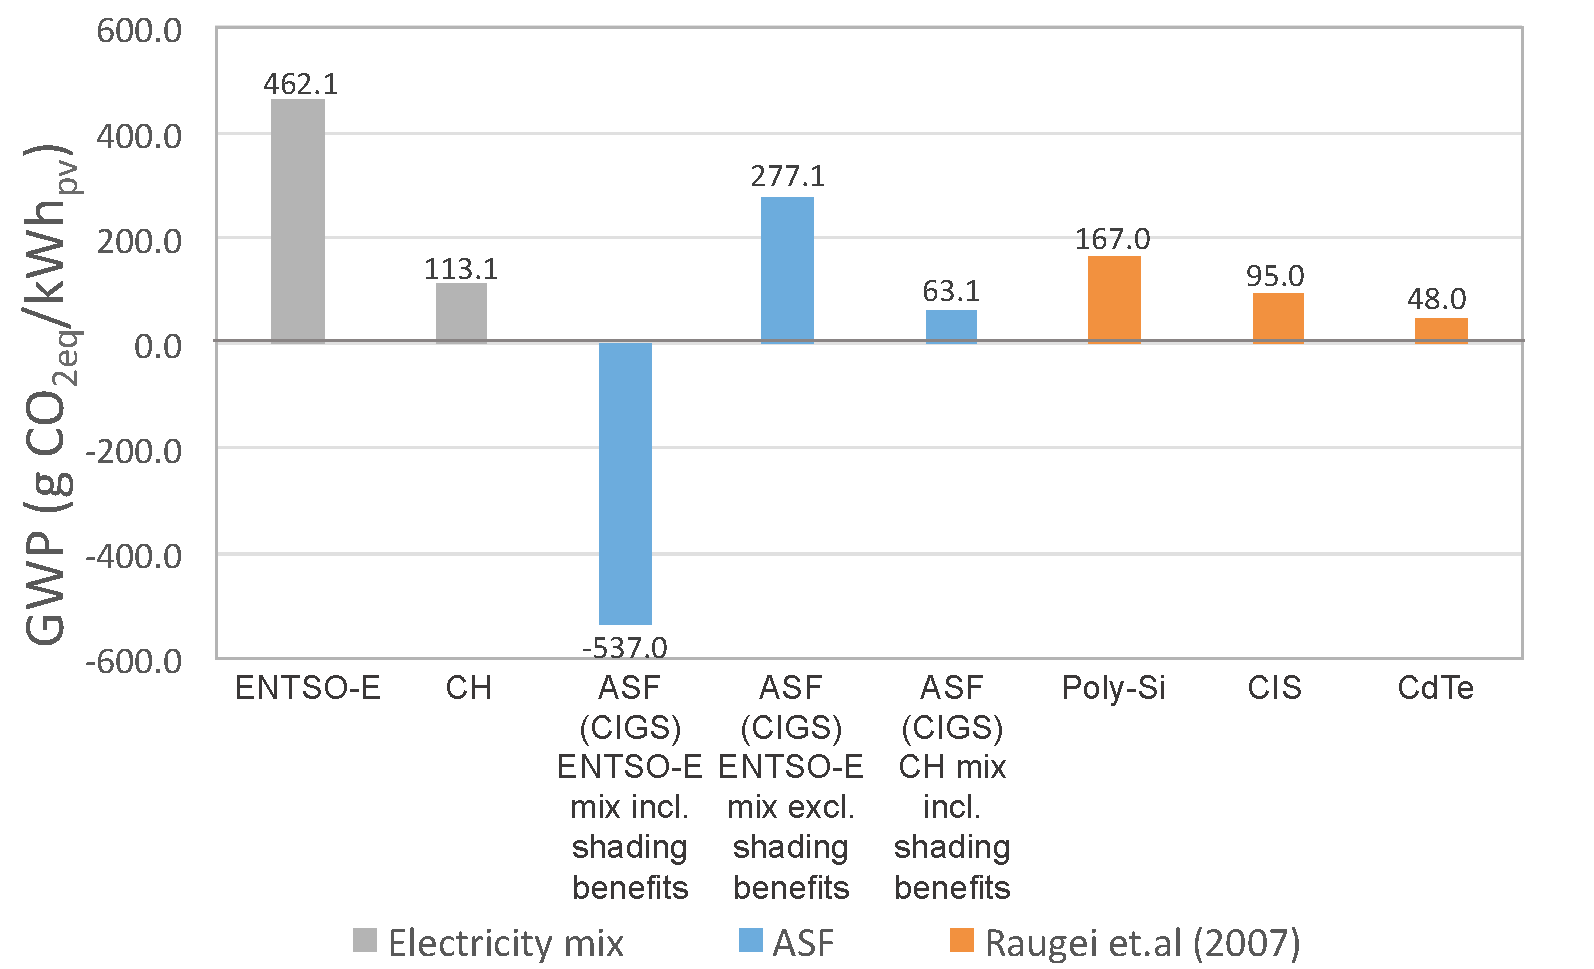
\includegraphics[width=10cm, trim= 0cm 0cm 0cm 0cm,clip]{compPV}
\caption{BIPV comparison of thin-film and BOS}
\label{fig:compPV}
\end{center}
\end{figure}


\begin{figure}[H]
\begin{center}
\includegraphics[width=10cm, trim= 0cm 0cm 0cm 0cm,clip]{louvres}
\caption{The comparison of the ASF with a static louvered shading system}
\label{fig:louvres}
\end{center}
\end{figure}
% I think I would prefer good old stacked bar plots


